\begin{figure}[H]
  \centering
  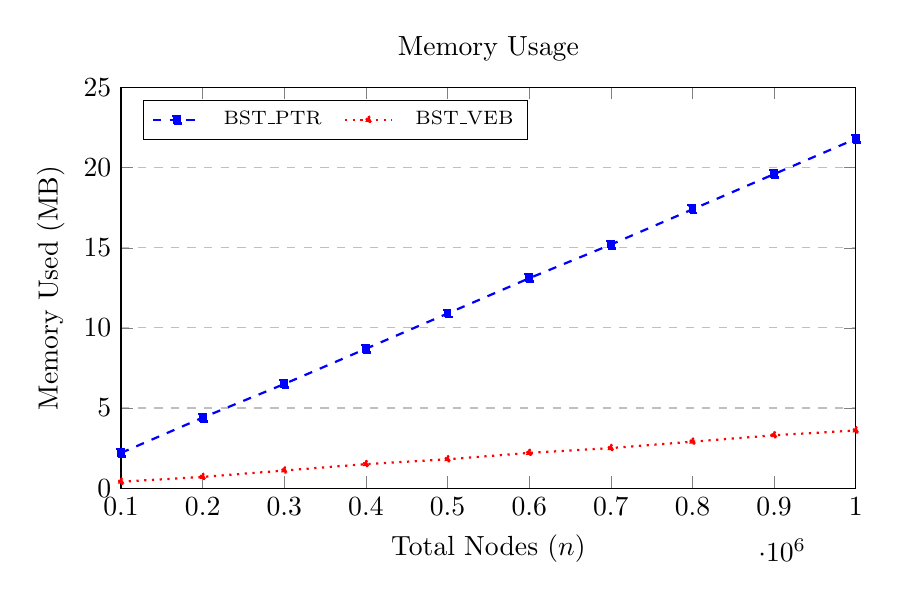
\begin{tikzpicture}
    \begin{axis}[
        title={Memory Usage},
        xlabel={Total Nodes ($n$)},
        ylabel={Memory Used (MB)},
        width =0.9\textwidth,
        height=0.55\textwidth,
        xmin=100000, xmax=1000000,
        ymin=0, ymax=25,
        ymajorgrids,
        grid style=dashed,
        legend columns=2,
        legend pos     = north west,
        legend style={font=\scriptsize, column sep=6pt},
    ]

    \addplot+[blue, thick, dashed, mark=square*, mark options={scale=.7,fill=blue}]
      coordinates {
        (100000,2.2) (200000,4.4) (300000,6.5) (400000,8.7)
        (500000,10.9) (600000,13.1) (700000,15.2) (800000,17.4)
        (900000,19.6) (1000000,21.8)
      };
    \addlegendentry{BST\_PTR}

    \addplot+[red, thick, dotted, mark=triangle*, mark options={scale=.7,fill=red}]
      coordinates {
        (100000,0.4) (200000,0.7) (300000,1.1) (400000,1.5)
        (500000,1.8) (600000,2.2) (700000,2.5) (800000,2.9)
        (900000,3.3) (1000000,3.6)
      };
    \addlegendentry{BST\_VEB}

    \end{axis}
  \end{tikzpicture}
  \caption{Memory usage in MB as a function of total nodes ($n$) for the pointer-based (\texttt{BST\_PTR}) and VanEmde-Boas (\texttt{BST\_VEB}) implementations.}
  \label{fig:memory}
\end{figure}
